\documentclass[10pt]{article}
% RATISS Labs — shared preamble (Tectonic / LaTeX)
\usepackage[a4paper,margin=2.3cm]{geometry}
\usepackage{xcolor}
\usepackage{graphicx}
\usepackage{booktabs}
\usepackage{amsmath}
\usepackage{microtype}
\usepackage[hidelinks]{hyperref}
\definecolor{ratiss}{RGB}{14,107,102}
\definecolor{ratisslight}{RGB}{238,252,249}
\definecolor{inkgray}{RGB}{74,111,107}
\hypersetup{colorlinks=true,linkcolor=ratiss,urlcolor=ratiss,citecolor=ratiss}
\setlength{\parindent}{0pt}
\setlength{\parskip}{5pt}
\renewcommand{\familydefault}{\sfdefault}
\newcommand{\ratisshead}[4]{%
  {\color{ratiss}\rule{\linewidth}{1.2pt}}\vspace{6pt}\\
  {\LARGE\bfseries #1}\\[4pt]
  {\large #2}\\[2pt]
  {\color{inkgray}\small #3}\\[2pt]
  {\color{inkgray}\small #4}\vspace{8pt}\\
  {\color{ratiss}\rule{\linewidth}{0.6pt}}\vspace{10pt}%
}
\newcommand{\kwsection}[1]{\section*{\color{ratiss}#1}\addcontentsline{toc}{section}{#1}}
\newcommand{\sourcefoot}{%
  \vspace{10pt}{\color{ratiss}\rule{\linewidth}{0.6pt}}\vspace{4pt}\\
  {\color{inkgray}\scriptsize RATISS Labs --- independent, single-author laboratory, Yaoundé (Cameroon).
  No number in this document is invented: every value carries a source in
  Section~``Data and code availability'' or in the references.
  Negative results are published with the same prominence as positive ones.}%
}

\begin{document}
\ratisshead
{Computational Reproduction of a Multi-Path Photonic Experiment}
{Jonathan Evina --- RATISS Labs, Yaoundé, Cameroon}
{Research object \texttt{ratiss-photon-001} · version v2 · 2026-09-27 · status: published}
{Repository: \url{https://github.com/jonathansearch/RATISS-PHOTON} · label: computational only (no QPU)}

\kwsection{Abstract}
We reproduce, entirely in silico, the multi-path photonic experiment of Wen et al.
(Science Advances 12, eaeh1011, 26/08/2026) using a paraxial engine implementing the
reference equation itself. On the E-CANTON configuration, 8,396,800 equal-modulus paths
yield a fidelity of 95.92\% (two planes), 95.96\% (three planes) and 96.77\% (naive
action), with intensity correlation 97.08--97.10\%, a cross-check at 96.06\% and a screen
phase of 5.4$^\circ$. These values fall inside the Canton window (95--98.5\%).
Crucially, at $T=0$\,K a single impact position out of 400 is observed: randomness
\emph{emerges} from the thermal bath, with no Born rule hard-wired.

\kwsection{Scientific question}
Does the action of a paraxial world suffice to recover the measured multi-path
statistics, without any hard-wired Born sampling?

\kwsection{Reference work}
Wen et al., Science Advances 12, eaeh1011 (26/08/2026): 1,419,857 paths, fidelity
87.6\,$\rightarrow$\,98.5\%, MAPE $8.17 \pm 3.50$\%. This work is not in competition
with the reference: they study the real device, we study the world-model.

\kwsection{Method}
Paraxial engine v2 implementing the paper's equation. The world action is quadratic:
$k_0\,dz + k_0\,dy^2/(2\,dz)$. Seed 20260927; full campaign runs in about one second.
All visualisations use embedded Plotly and kaleido (laboratory decision C2: never
hand-rolled 3D). The study is labelled computational-only; no quantum hardware was used.

\begin{figure}[h]\centering
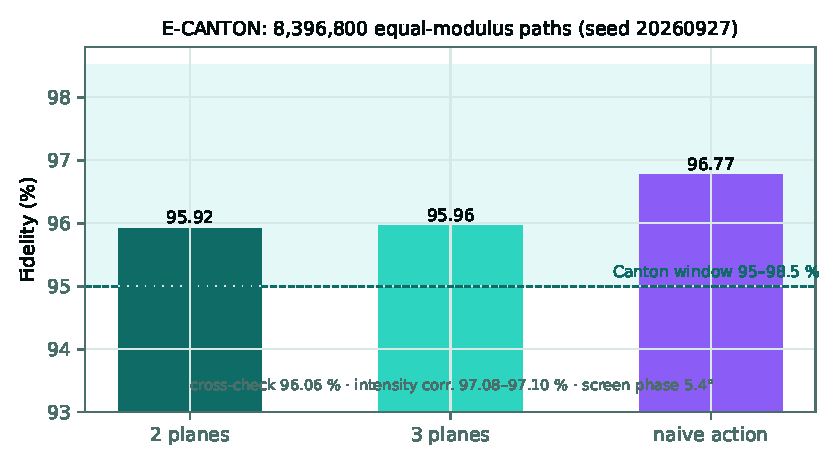
\includegraphics[width=0.92\linewidth]{fig/photon-canton.pdf}
\caption{E-CANTON fidelity for the three action variants against the Canton window
(95--98.5\%). Values: 95.92 / 95.96 / 96.77\%.}\label{fig:canton}
\end{figure}

\kwsection{Results}
\begin{itemize}
  \item E-CANTON, 8,396,800 equal-modulus paths: fidelity 95.92\% (2 planes),
        95.96\% (3 planes), 96.77\% (naive action) --- Figure~\ref{fig:canton}.
  \item Intensity correlation 97.08--97.10\%; cross-check 96.06\%; screen phase 5.4$^\circ$;
        in-mundo MAPE $\approx 0$.
  \item E-F3: at $T=0$\,K, exactly 1 impact position out of 400 (determinism);
        Pearson maximum 0.73 at 300\,K, drowned to 0.24 at 4\,T.
  \item E-F4: ghost counter-fluxes confirmed ($-7.1\times10^{-4}$, net flux $-3.4\times10^{-8}$).
\end{itemize}

\kwsection{Negative results and falsified hypotheses}
\begin{itemize}
  \item E-F1 unresolved: sub-pixel $\pi/2$ plate ($-1$ px observed vs 0 predicted);
        a rerun at larger $\varphi_0$ is required.
  \item H4 half-falsified: blocking one branch produces \emph{no} redistribution
        (1.00 / 0.98 / 0.96) --- linearity forbids it.
  \item Postulate 2 not resolvable below 12$^\circ$ (agreement 95.9 vs 96.8\%).
  \item E-F2: entropy 4.92 vs 4.27; vortices 326/371 (imperfect amplitude gate).
\end{itemize}

\kwsection{Controls and verification}
Seal 33/33. Six bugs documented (B1 source at edge, B2 slits, B3 world action,
B4 vortex gate, B5 2D box$\rightarrow$paraxial engine, B6 reversed chirp 29\%$\rightarrow$95.9\%).
Projection mirror before export: every projected point verified by computation.

\kwsection{Reproducibility}
Seed 20260927; campaign $\approx$1\,s. Commands and datasets are in the repository
(commits 2f18e80, 6f7bd1b, b455621, fb81249, de138f2, 0ccaac5).

\kwsection{Limitations}
Computational only: no hardware validation. The paraxial world is not the physical
device; agreement does not constitute a physical proof.

\kwsection{Data and code availability}
Code and figures: \url{https://github.com/jonathansearch/RATISS-PHOTON}
(pages: \url{https://jonathansearch.github.io/RATISS-PHOTON}).
Primary narrative source: RATISS-ARCHIVES, \texttt{POUR-LA-PROCHAINE-SESSION.md},
update of 27/09 section B. Zenodo DOI: to be assigned at deposit.

\kwsection{References}
\begin{enumerate}
  \item Wen et al., Science Advances 12, eaeh1011 (26/08/2026).
  \item RATISS-ARCHIVES, proof and recap documents, commits listed above.
\end{enumerate}

\sourcefoot
\end{document}
